\documentclass{beamer}
%\setbeameroption{show notes on second screen=right} % Both
\setbeameroption{hide notes} % Only slides
%\setbeameroption{show only notes} % Only notes
% Theme choice:
\usetheme{Berlin}
\usepackage{tikz}
\usepackage{tikz-feynman}
\usepackage{animate}
\usepackage{amsmath}
\usepackage{cancel}
\usepackage{multicol}
\usepackage{physics}
\usepackage{graphicx}
\usepackage{amsfonts}
\usepackage{caption}
\usepackage{wrapfig}
\usepackage{pgfplots}
\usepackage{subfigure}
\newcommand{\semitransp}[2][35]{\textcolor{fg!#1}{#2}}
\pgfplotsset{compat=1.15}
\captionsetup{singlelinecheck=false}
\usefonttheme[onlymath]{serif}
\usepgfplotslibrary{fillbetween}
\pgfmathdeclarefunction{gauss}{2}{%
	\pgfmathparse{1*exp(-((x-#1)^2)/(2*#2^2))}%
}

%\usepackage{hyperref}
%\hypersetup{colorlinks = true,linkcolor = black,filecolor= black,urlcolor= black}
%\usepackage{subcaption}
\usepackage[backend=bibtex,bibencoding=utf8,doi=false,isbn=false,url=false,eprint=false,indexing=false,style=authoryear]{biblatex}
\addbibresource{library}
\AtEveryBibitem{%
	\clearname{translator}%
	\clearlist{publisher}%
	\clearfield{pagetotal}%
}
\usepackage{MnSymbol,wasysym}
\usepackage[toc,page]{appendix}
\usetikzlibrary{snakes}
\usetikzlibrary{shapes.geometric, calc}
\author{Vo Chau Duc Phuong}
\institute[ICTP]{The Abdus Salam International Center for Theo retical Physics}
% Title page details: 
\title[Introduction To Quantum Hall Effect]{Introduction To Quantum Hall Effect}
\begin{document}
	\begin{frame}
		\titlepage
	\end{frame}
	\begin{frame}{Table of Contents}
		\tableofcontents
	\end{frame}
	\section{The Classical and Quantum Hall Effect}
\begin{frame}{The Classical Hall Effect}
\begin{columns}
	% Column 1
	\begin{column}{0.5\textwidth}
\quad The equilibrium of the Hall effect can be described using Ohm's law in convention:
$$\begin{pmatrix}
	E_x\\E_y
\end{pmatrix}
= \begin{pmatrix}
	\rho_{xx} & \rho_{xy}\\
	-\rho_{xy} & \rho_{yy}
\end{pmatrix}
\begin{pmatrix}
	J_x\\0
\end{pmatrix},$$
	\end{column}
	% Column 2    
	\begin{column}{0.5\textwidth}
		\begin{figure}
			\centering
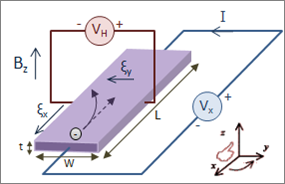
\includegraphics[width=0.7\textwidth]{Images/Hall effect.png}
\label{fig: Ohm clas}
\caption{Classical Hall effect}

		\end{figure}
	\end{column}
\end{columns}
\vspace{-0.3cm}in which:
$$	\rho_{xy} = \frac{E_y}{J_x} = -\frac{B}{ne},\qquad
	\rho_{xx} = \frac{E_x}{J_x} = \frac{m}{ne^2 \tau}$$
Classically:
\begin{center}
	\(E_y \propto B\) and \(E_x\) depend on scattering parameter \(\tau\)
\end{center}
\end{frame}
\begin{frame}{The Quantum Hall Effect}
\quad First introduced in 1980 \footcite{Kitzling_1980} and later on being investigated, The resistance in a MOSFET under a strong magnetic field shows interesting properties:\null\\
\begin{columns}
	%col1
\begin{column}{0.5\textwidth}
\\
\quad At certain point:
\begin{align*}
	\rho_{xx} &= 0.\\
	\rho_{xy} &\sim \frac{1}{\nu}, \quad \nu \in \mathbb{N}
\end{align*}
\quad Between these points:
$$\rho_{xy} = const.$$
\end{column}
	%col2
\begin{column}{0.5\textwidth}
\begin{figure}
	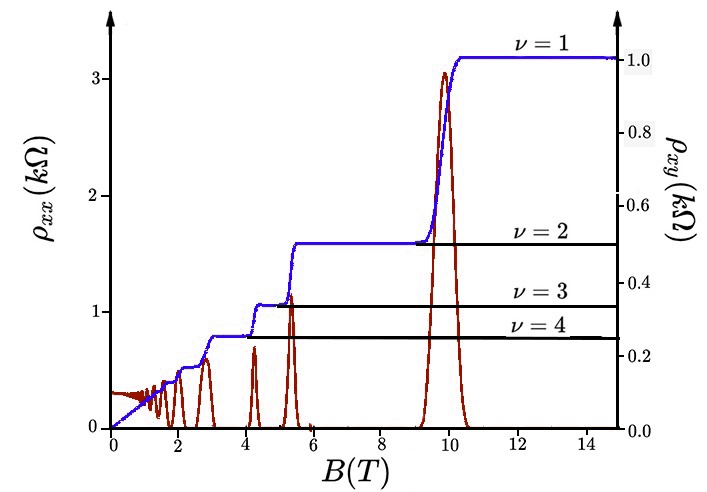
\includegraphics[width=0.8\linewidth]{Images/Rhoxy.jpg}
\caption{Quantum Hall Resistance
	\cite*[Taken from ][]{manchesterAdvancedQuantum}}
\label{Fig: QHE}
\end{figure}
\end{column}
\end{columns}
\begin{center}
\end{center}
\end{frame}
\begin{frame}
\quad Therefore, we will explain this effect as:
\begin{itemize}
	\item Why does \(\rho_{xx} \to 0\) is a peaks at some certain points and \(0\) otherwise?
	\item Why these plateux exist?
\end{itemize}
\end{frame}
	\section{Landau Levels}
\begin{frame}
\quad For a 2D electron gas in an external field field \(\textbf{B} = (0,0,B)\) \& \(\textbf{E} = (E,0,0)\). If we choose Landau gauge \(\textbf{A} = (0,Bx,0)\), the eigenstates will be the Landau levels with the energy:
\begin{equation}\label{Eq: Landau or}
	E_{{\color{blue} \nu},{\color{red}k_y}} = \hbar \omega_B\bigg({\color{blue} \nu} + \frac{1}{2}\bigg) - eE\bigg({\color{red}k_y}l_B^2 + \frac{eE}{m\omega_B^2}\bigg) + \frac{m}{2}\frac{E}{B},
\end{equation}
\begin{columns}
	
\begin{column}{0.4\textwidth}
in which
\begin{equation*}
	\omega_B = \frac{eB}{m},\quad l_B = \frac{\hbar}{eB}
\end{equation*}
\quad Recover the classical drift along \(\textbf{E} \cross \textbf{B}\) direction:
\begin{equation}\label{eq: vy}
v_y = \frac{1}{\hbar} \pdv{E_{\nu,k_y}}{k_y} = -\frac{E}{B}
\end{equation}
\end{column}
\begin{column}{0.6\textwidth}
\begin{figure}
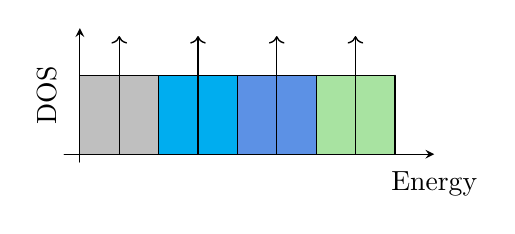
\begin{tikzpicture}[line cap=round,line join=round]
\definecolor{grannysmithapple}{rgb}{0.66, 0.89, 0.63}
\definecolor{unitednationsblue}{rgb}{0.36, 0.57, 0.9}
\begin{axis}[ticks=none, x=1cm,y=1cm, axis lines=middle, xmin=-0.2, xmax=4.5, ymin=-0.1,x label style={at={(axis description cs:1,0)},anchor=north}, y label style={at={(axis description cs:-0.1,0.5)},rotate=90},ymax=1.6,xlabel=Energy,ylabel=DOS]
\filldraw[draw=black,fill=lightgray] (0.,0.) rectangle(1.,1.);
\filldraw[draw=black,fill=cyan] (1,0) rectangle (2,1);
\filldraw[draw=black,fill=unitednationsblue] (2,0) rectangle (3,1);
\filldraw[draw=black,fill=grannysmithapple] (3,0) rectangle (4,1);
\draw [->,line width=0.5pt] (0.5,0) -- (0.5,1.5);
\draw [->,line width=0.5pt] (1.5,0) -- (1.5,1.5);
\draw [->,line width=0.5pt] (2.5,0) -- (2.5,1.5);
\draw [->,line width=0.5pt] (3.5,0) -- (3.5,1.5);
	\draw [line width=0.5pt] (4,1)-- (4,0);
\end{axis}
	\end{tikzpicture}
\caption{From constant DOS to Dirac comb}
\end{figure}
\end{column}
\end{columns}
\end{frame}
\begin{frame}{Conductivity}
\quad Each filled Landau levels have the degeneracy (in this convention, it's \({\color{red} k_y}\)) that when we take over the sum to get:
$$\textbf{I} = -e \ev{\dot{\textbf{x}}} = - e \sum_{n = 1}^\nu \sum_{k_y} \ev{\frac{\hbar}{i}\nabla - \textbf{A}}{\psi_{n k_y}}$$
\begin{equation}\label{eq: Ixy}
	\Rightarrow \qquad I_x = 0,\qquad I_y = -\sum_{k_y}e\nu\frac{E}{B} = \frac{e^2 \nu E}{2\pi \hbar}$$
	This result in:
	$$\rho_{xx} = 0, \qquad\rho_{xy} = \frac{2\pi \hbar}{e^2 \nu},
\end{equation}
in which \(\nu\) is the total filled number of Landau levels.
\end{frame}
	\section{The Importance of Impurity and Edge states}
\begin{frame}
\begin{center}
	But these conduction above not explained everything!
\end{center}
Revisit the calculation of \eqref{eq: Ixy} from \eqref{eq: vy} with a more generalize approach (Taylor expand \(V(x)\) up to first order) give:
%\begin{columns}
%	\begin{column}{0.5\linewidth}
		\begin{align}
			v_y &= - \frac{1}{eB} \pdv{V(x)}{x}\\
			\sigma_{xy} = \frac{E_y}{I_x} &=\sum_\nu \frac{e}{E L_x}\int\frac{dk}{2\pi} v_y (x) \nonumber\\&=\sum_\nu \frac{e}{\cancel{E L_x}}\frac{\cancel{V(x_{max}) - V(x_{min})}}{2\pi \hbar} = \frac{\nu e^2}{2\pi\hbar}
		\end{align}
Invert: $$\rho_{xy}\propto 1/\nu$$
%	\end{column}
%\begin{column}{0.5\linewidth}
%	\begin{figure}[!ht]\centering
%		\begin{tikzpicture}
%			\coordinate (a) at (-1,0.5);
%			\coordinate (b) at (1,0.5);
%			\coordinate (a1) at (-1.5,1.5);
%			\coordinate (b1) at (1.5,1.5);
%			\draw[thick,->] (-2,0) -- (2,0)node[anchor= north west] {\(x\)} ;
%			\draw[thick,->] (0,-0.4) -- (0,2)node[anchor= north east]{\(V(x)\)};
%			\draw [thick, red,rounded corners=0.6mm] (-1.54,1.6) -- (a1) --(-1.1,0.52)-- (a)  --  (b) -- (1.1,0.5) --(b1);
%			\draw[dashed] (-1.45,1.4)node[anchor= south east] {} -- (0,1.4);
%			\draw[dashed] (1.35,1.08)node[anchor= south west] {} -- (0,1.08) node[anchor= south west]  {\(\Delta V\)};
%		\end{tikzpicture}
%		\caption{\centering Difference in Fermi energy at both sides Edge's potential \(V(x)\)}
%	\end{figure}
%\end{column}
%\end{columns}
\vspace{0.3cm}
$\Rightarrow$ As long as the \(\partial_x V(x)\) smooth enough, only the difference of the edges create the quantize value!
\end{frame}
\begin{frame}
\small{But, why are the plateaus rounded rather than sharp, as seen in Fig. \ref{Fig: QHE}?}\\\vspace{0.05cm}
{\centering $\Rightarrow$ It turns out that disorder (impurities) play a crucial role!}\\\vspace{0.05cm}
\begin{columns}
\begin{column}{0.6\linewidth}
Disorder causes:\null
\begin{itemize}
\item Perturbation \(\to\) Broader side (peaks!).\\
\item \semitransp{Catch the localized state \(\to\) Plateaus!}
\end{itemize}
\vspace{0.2cm}
The Impurity act as a perturbation, causing the broad edge of the energy.\vspace{0.2cm}
\begin{center}
Sample too perfect? \(\to\) flat spectrum
\end{center}
\vspace{0.2cm}
But:
\end{column}
\begin{column}{0.4\linewidth}
	\begin{figure}
\subfigure[{\small Without disorder}]{\scalebox{0.8}{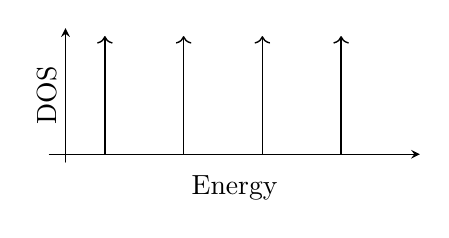
\begin{tikzpicture}[line cap=round,line join=round]
\definecolor{grannysmithapple}{rgb}{0.66, 0.89, 0.63}
\definecolor{unitednationsblue}{rgb}{0.36, 0.57, 0.9}
\begin{axis}[ticks=none,x=1cm,y=1cm,axis lines=middle,xmin=-0.2052410812264766,xmax=4.5,ymin=-0.1,x label style={at={(axis description cs:0.5,-0.03)},anchor=north}, y label style={at={(axis description cs:-0.06,0.5)},rotate=90},
ymax=1.6,xlabel=Energy,ylabel=DOS]
\draw [->,line width=0.5pt] (0.5,0) -- (0.5,1.5);
\draw [->,line width=0.5pt] (1.5,0) -- (1.5,1.5);
\draw [->,line width=0.5pt] (2.5,0) -- (2.5,1.5);
\draw [->,line width=0.5pt] (3.5,0) -- (3.5,1.5);
\end{axis}
\end{tikzpicture}}}\qquad
\subfigure[{\small with disorder}]{\scalebox{0.8}{\begin{tikzpicture}[line cap=round,line join=round]
\begin{axis}[every axis plot post/.append style={mark=none,domain=-2:4,samples=100,smooth},ticks=none,x=1cm,y=1cm,axis lines=middle,xmin=-0.2052410812264766,xmax=4.5,ymin=-0.1,x label style={at={(axis description cs:0.5,-0.03)},anchor=north}, y label style={at={(axis description cs:-0.06,0.5)},rotate=90},
ymax=1.6,xlabel=Energy,ylabel=DOS]
\addplot[color=black] {gauss(0.5,0.1)};
\addplot[color=black] {gauss(1.5,0.1)};
\addplot[color=black] {gauss(2.5,0.1)};
\addplot[color=black] {gauss(3.5,0.1)};
\addplot[color=black] {gauss(4.5,0.1)};
\end{axis}
\end{tikzpicture}}}
	\end{figure}
\end{column}
\end{columns}
\begin{center}
	Too much disorder \(\to\) not recognize the peaks!
\end{center}
\end{frame}
%\begin{frame}
%Revisit the current resistance from solid state physics:
%\begin{itemize}
%\item Fully filled band levels can't give electric current. $\to$ insulator\\
%\item Partly filled band levels only give current that only can measured if there are the present of disorder (impurity) 
%\end{itemize}
%The idea is somewhat alike, in quantum Hall effect:
%\begin{itemize}
%	\item Filled bands give insulation.
%	\item Disorder (impurity) is a key!
%\end{itemize}
%\end{frame}
\begin{frame}
\quad From the calculation of the Landau levels \eqref{Eq: Landau or}, there's the degeneracy \(k_y\) in each Landau levels \(\nu\):
\begin{columns}
\begin{column}{0.5\linewidth}
\begin{itemize}
\item Decrease B $\to$ more bands filled
\item Total number of electrons: constant
\end{itemize} 
\only<2>{But:
	\begin{itemize}
		\item Same filled levels \(\nu\): \(N_e \propto B\).\\
	\end{itemize}
\begin{center}
	Where do the electrons go?\\
They're still there!\\(just not in the bands!)
\end{center}}
\end{column}
\begin{column}{0.5\linewidth}
\only<1>{\begin{figure}
	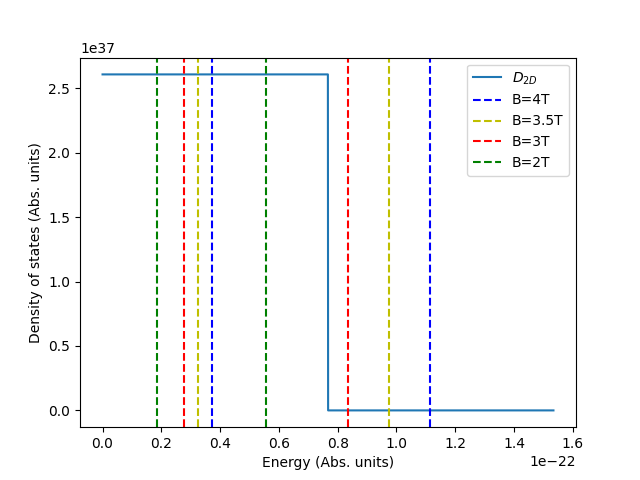
\includegraphics[width = \linewidth]{images/decreseB.png}
\caption{Illustrated number of filled levels when decrease \(B\)}
\end{figure}}
\only<2>{\begin{figure}
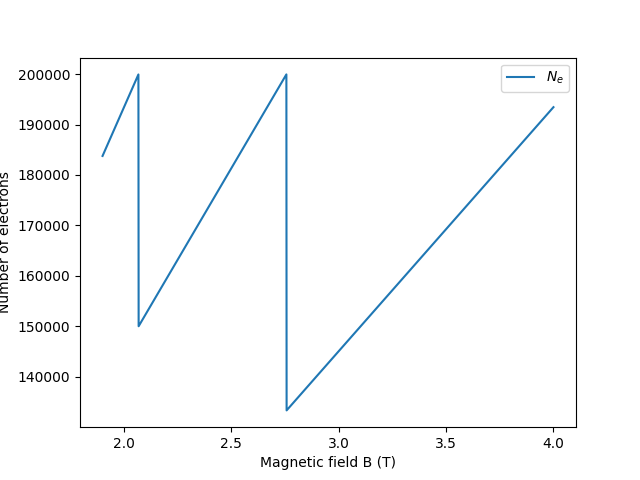
\includegraphics[width = \linewidth]{images/Ne.png}
\caption{Illustrating number of electrons accommodated in Landau level when decreasing \(B\)}
\end{figure}}
\end{column}
\end{columns}
\end{frame}
\begin{frame}
	\begin{columns}
		\begin{column}{0.6\linewidth}
			Disorder causes:\null
			\begin{itemize}
				\item Perturbation \(\to\) Broader side (peaks!).\\
				\item Catch the localized state \(\to\) Plateux!
			\end{itemize}
			\vspace{0.2cm}
The impurity \(\to\) broad peaks (higher or lower energy than the center)\(\to\) localized by the impurity\vspace{0.1cm}
			\begin{center}
Localized state don't contribute in conduction \(\to\) plateux
			\end{center}
		\end{column}
		\begin{column}{0.4\linewidth}
\begin{figure}
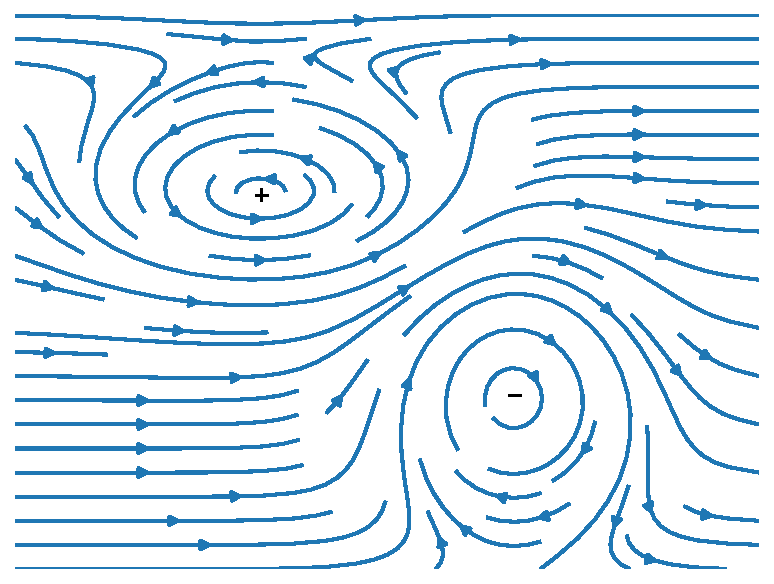
\includegraphics[width = \linewidth]{images/Disorder.pdf}
\caption{Movement of center of mass localized under impurity's maximum \(+\) or minimum \(-\).}
\end{figure}
		\end{column}
	\end{columns}
\vspace{0.2cm}
When decrease \(B\) but not filled the next level yet:
	\begin{center}
	\(\to\) The electrons will populate the localized states!
	\end{center}
\end{frame}
\begin{frame}{The Quantum Hall Effect}
	\quad So, let summary two main aspects:\null\\
	\begin{columns}
		\begin{column}{0.5\textwidth}
\begin{itemize}
\item Edge states make sure quantized values.\\ 
\item Impurity create the peaks and the plateux.\\
\end{itemize}
\quad Partly filled levels?\\
$\rightarrow$ Impurity create scattering inside level $\to$ longitude peaks.
		\end{column}
		%col2
		\begin{column}{0.5\textwidth}
			\begin{figure}
				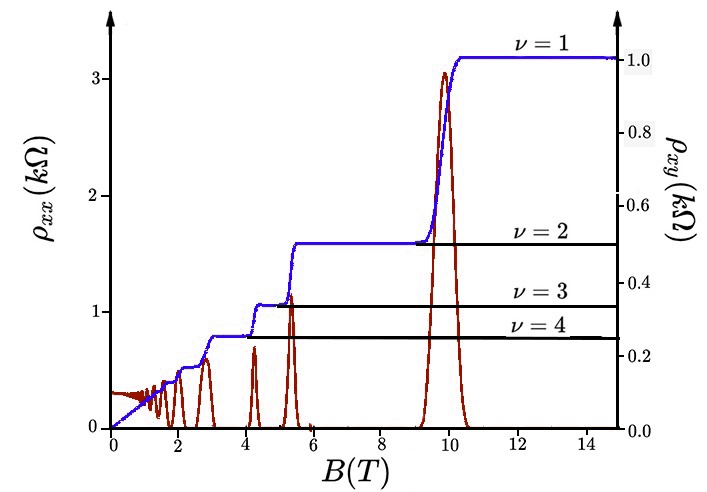
\includegraphics[width=0.8\linewidth]{Images/Rhoxy.jpg}
				\caption{Quantum Hall Resistance
					\cite*[Taken from ][]{manchesterAdvancedQuantum}}
			\end{figure}
		\end{column}
	\end{columns}
\end{frame}
\begin{frame}
So, what do the edge states have to do with the topology?\\\vspace{0.2cm}
These states enable a "highway current" that flows along the boundaries of the sample without backscattering, even in the presence of impurities.\\\vspace{0.2cm}
Therefore, as long as the currents:
\begin{itemize}
\item  not cut on the other (change the topology).
\item stay non-localized, no back scattering.
\item remain well-separated to prevent tunneling.
\end{itemize}
The system will exhibit quantized conductance and dissipationless transport.
\begin{center}
	Everything have been explained! Or not?
\end{center}
\end{frame}
\begin{frame}{Beyond The Integer}
	\begin{figure}
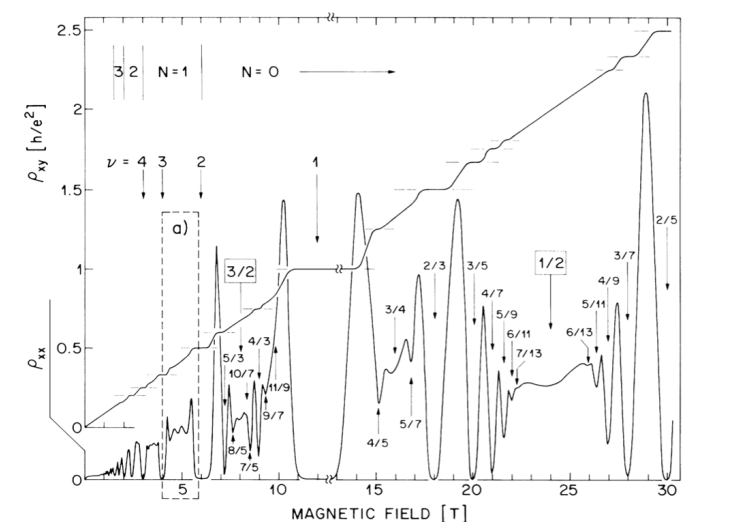
\includegraphics[width =0.7\linewidth]{images/FQH.png}
\begin{center}
	\caption{Fraction Hall Effect, from David Tong's lecture notes}
\end{center}
	\end{figure}
\end{frame}
\begin{frame}[c]
	\begin{center}
Thank you for your listening.
	\end{center}
\end{frame}
\begin{frame}
Reference:
\printbibliography
\end{frame}
\end{document}
